\section{Global Sharding Protocol}
\label{section:sharding}

\paragraph{\mainshard.}
The first shard, known as the \mainshard, 
 holds essential data about the protocol's consensus 
 and its current parameters.
It also contains information about other shards 
 and the hashes of the most recent replication packets from all shards.
Finally, it is responsible for mapping accounts to their corresponding execution shards.
In essence, the \mainshard serves a dual purpose:
\begin{itemize}
    \item It sets the protocol's rules and parameters.
    \item It ensures synchronization across all other shards, 
     including verifying state transition proofs from these shards.
\end{itemize}

% \todo[inline]{Define the \mainshard's outer interface: zk, da, and other components}

\paragraph{Execution Shards.}

Execution shards are responsible for processing user transactions.
Each shard manages a predefined subset of accounts.
The assignment of accounts to shards is determined by a mapping, which is stored on the \mainshard:
\[
    F_S: a \mapsto \texttt{shardId}
\]
In this context, $a$ represents the account's address,
 while $F_S$ directly maps this key to a shard identifier.
This mapping can be manually updated by users' requests, subject to constraints
 maintained by the colocation manager, as detailed in the section \ref{section:colocation}.

Each shard is maintained by a specific group of validators (\textit{committee}).
These validators run a "local" consensus algorithm 
 to ensure the shard's state consistency. 
Details about the shard's local consistency are provided in Section \ref{section:local-consensus}.


\subsection{Validators Rotation Procedure}
\label{setion:validators-rotation}

At the end of each epoch, the whole validator set generates a new seed for the next epoch using a Verifiable Secret Sharing (VSS) scheme \cite{VSS,RapidChain}.
The seed is used by the validators to generate a new committee for each shard.
$$
\texttt{assignment} : \texttt{shardIds} \to 2^\texttt{validators}
$$
The exact mechanism of assignment update:
\begin{enumerate}
\item For each \texttt{shardId}, an array of the following values is sorted
$$
\texttt{PRF}_{\texttt{seed}}(\texttt{shardId} || \texttt{validatorId})
$$
\item The validators corresponding to the first $n$ values are used to form a new committee for the shard.
\end{enumerate}

One could rotate leaders in a round-robin fashion, $\texttt{leader\_id} = \texttt{view} \mod n$,
but this would be vulnerable to DoS attacks, since an adversary easily can obtain the leader schedule.
A leader election protocol based on Verifiable Random Functions (VRFs), as proposed in \cite{LibraBFT}, is utilized:
\begin{align*}
    \texttt{seed} &= \texttt{VRF}_{\texttt{prev\_leader}}(\texttt{height}, \texttt{view}) \\
    \texttt{leader\_id} &= \texttt{PRF}_{\texttt{seed}}(\texttt{view}) \mod n
\end{align*}
where \texttt{PRF} is a pseudorandom function.
The leader of the previous view provides the seed as a result of evaluating the VRF.
Every node can verify that the seed is correct by evaluating the VRF with the public key of the previous leader.

\subsection{Cross-Shard Communication}
\label{section:cross-shard}

As previously highlighted, all accounts are distributed among shards. 
At an initial glance, this might seem similar to the data fragmentation issue 
found in the application-specific rollups approach. 
However, the key difference is in how cross-shard communication is handled: 
it's integrated directly into the overall protocol, 
rather than being managed by separate bridges. 

In zkSharding, processing of transactions across shards is mediated by cross-shard transactions (CSTs). 
To constrain the manipulation and exploitation of CST processing, ZkSharding employs a directed acyclic graph (DAG) architecture called the shardDAG that combines protocol rules, rewards and penalties to incentivise and define a verifiable order in which CSTs must be processed.
Within each shard, this order roughly corresponds to processing CSTs in the order in which they were created, completing any existing CSTs before new transactions can be initiated.

The strategy for achieving constraints and to guarantee eventual transaction processing is shown in Fig.~\ref{figure:shardDAGStrategy}. 
\begin{figure}[h!]
	\centering
	
\includegraphics[width=1.0\textwidth]{figures/shardDAGStrategy.jpg}
	\caption{Achieving constraints on transaction exploitation and guaranteeing eventual transaction processing requires enforceable protocol rules for ordering of transaction and CST processing.
		An enforceable order requires enforcing shards to receive CST data from other shards. 
		Enforcing receipt of CST data requires enforcing that the CST data is available. 
		Thus, exploitation constraints and eventual transaction processing rests upon data availability of CSTs.}
	\label{figure:shardDAGStrategy}
\end{figure}

A key outcome of the shardDAG is the guarantee that once a block containing cross-shard transactions is included in a (valid) consensus block, then those cross-shard transactions are guaranteed to (eventually) be processed and included in their destination shards. 
Therefore, all transactions are guaranteed to be processed once they have begun processing in an initial shard.

Figure~\ref{figure:order-example} illustrates how the shardDAG induces an order of transaction and cross-shard transaction processing via a simple example shardDAG on the left. 
In this example shard $B$ block 2 is in the process of being created using hashes to its prior block shard $B$ block 1, as well as shard $C$ block 1 and consensus block 0. 
Coloured parts of blocks indicate CSTs with destination shard B.
In this example is assumed that all cross-shard transactions are pending (i.e. not included in shard $B$ block 1 or earlier). 
Tracing the DAG edges allows most (but not all) pairs of blocks to be ordered with respect to each other.
The centre of the figure shows a partial order of shard blocks in shard $B$ block 2’s subgraph.
The order in which CSTs are included in shard $B$ block 2 must be consistent with the partial ordering of shard blocks. 
Two example valid shard $B$ block 2's are shown.
Notice that any new transactions ($b2$) can only be included after any CSTs, i.e. transactions that are partially processed are prioritised over new transactions.
Shard block proposers can select the order of cross-shard transactions amongst blocks that are equally ordered e.g. the red and blue CSTs. 
If block capacity restricts inclusion, only the earliest cross-shard transactions are included in shard $B$ block 2, any remaining unprocessed CSTs will be processed in later blocks.

\begin{figure}
	\centering
	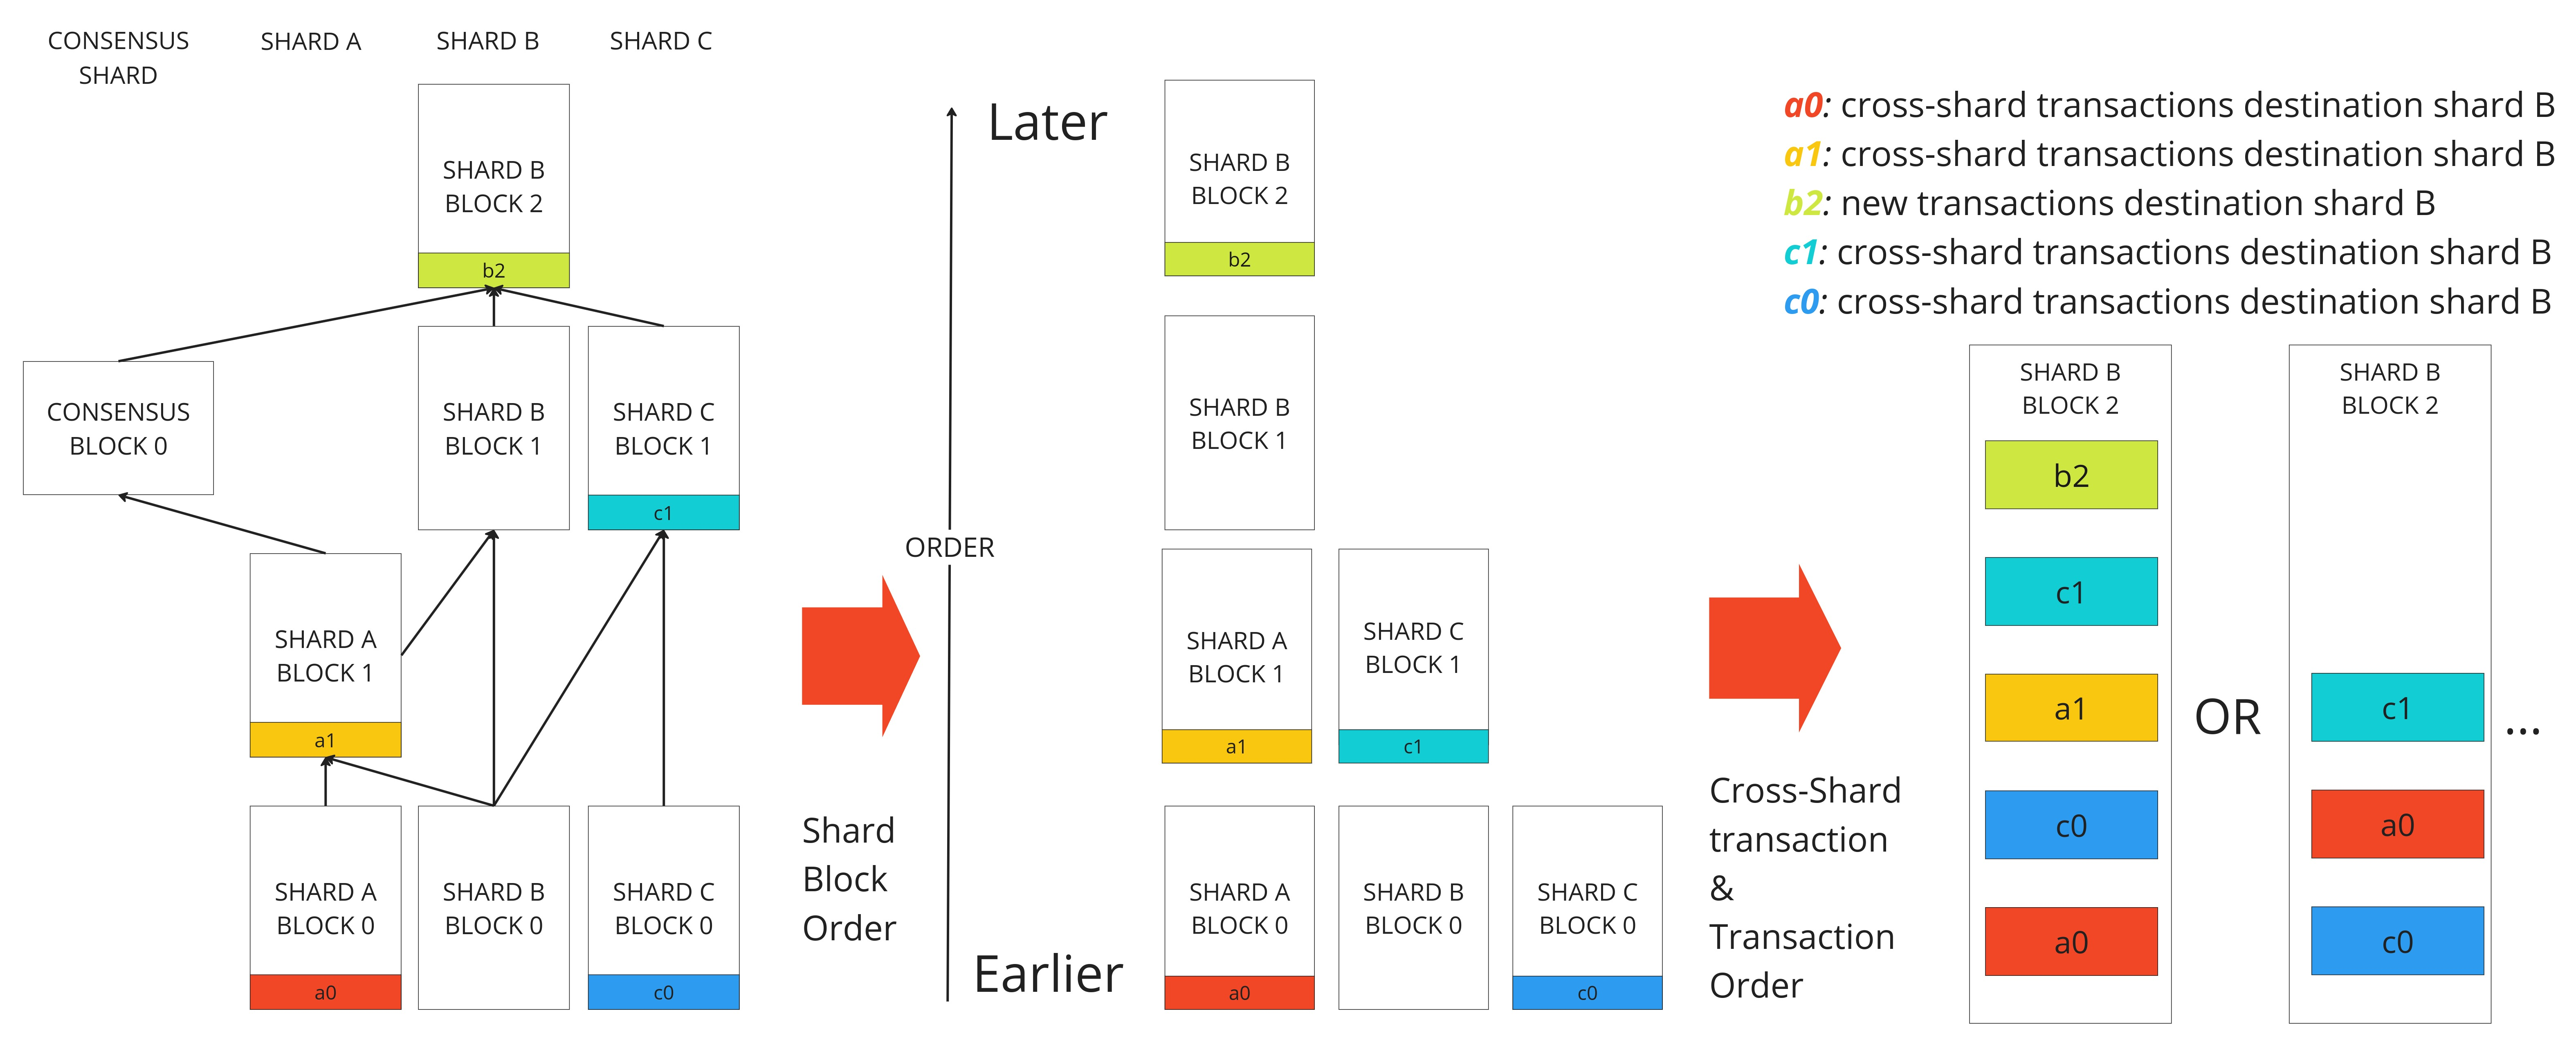
\includegraphics[width=1.0\textwidth]{figures/OrderExample.jpg}
	\caption{Left: Shard $B$ block 2's shardDAG subgraph.
		Centre: A partial order of shard blocks in shard $B$ block 2's subgraph.
		Right: The order of CST and transaction inclusion in a block must be consistent with the partial ordering of shard blocks.
		Two examples of valid shard $B$ block 2 are shown containing ordered CSTs. }
	\label{figure:order-example}
\end{figure}

\subsubsection{Shard DAG Formation}
To form a shardDAG shard blocks include
\begin{itemize}
	\item A hash to the previous (valid) shard block in the same shard, as in a typical blockchain.
	\item A set of hashes to other shards blocks in other shards.
	Up to $N-1$ hashes are allowed, where $N$ is the number of shards. 
	At most one hash per shard is allowed, and no hash can fall in the subgraph of another hash, to eliminate redundant data.
	\item a hash to a (valid) consensus block, equal to or later than the most recent consensus block already included in prior shard blocks.	
\end{itemize}
The subgraph of a shard block $b$ includes all shard blocks that can be reached starting from $b$ (including $b$ itself) by traversing edges in the shardDAG, including edges to and from consensus blocks.
An example shardDAG subgraph is shown in Fig.~\ref{figure:shard-formation}. 
The black block’s header contains a list of hashes (thick solid arrows) to its prior shard block in shard 1, another shard block in shard 2, and a single hash to a consensus block. 
The dotted arrow indicates a hash that is not allowed because the lower block is in the subgraph of a higher shard block, and the edge is therefore redundant. 
Thin arrows trace the subgraph of the black block, beyond the blocks explicitly included in its header via hashes. 


\begin{figure}
	\centering
	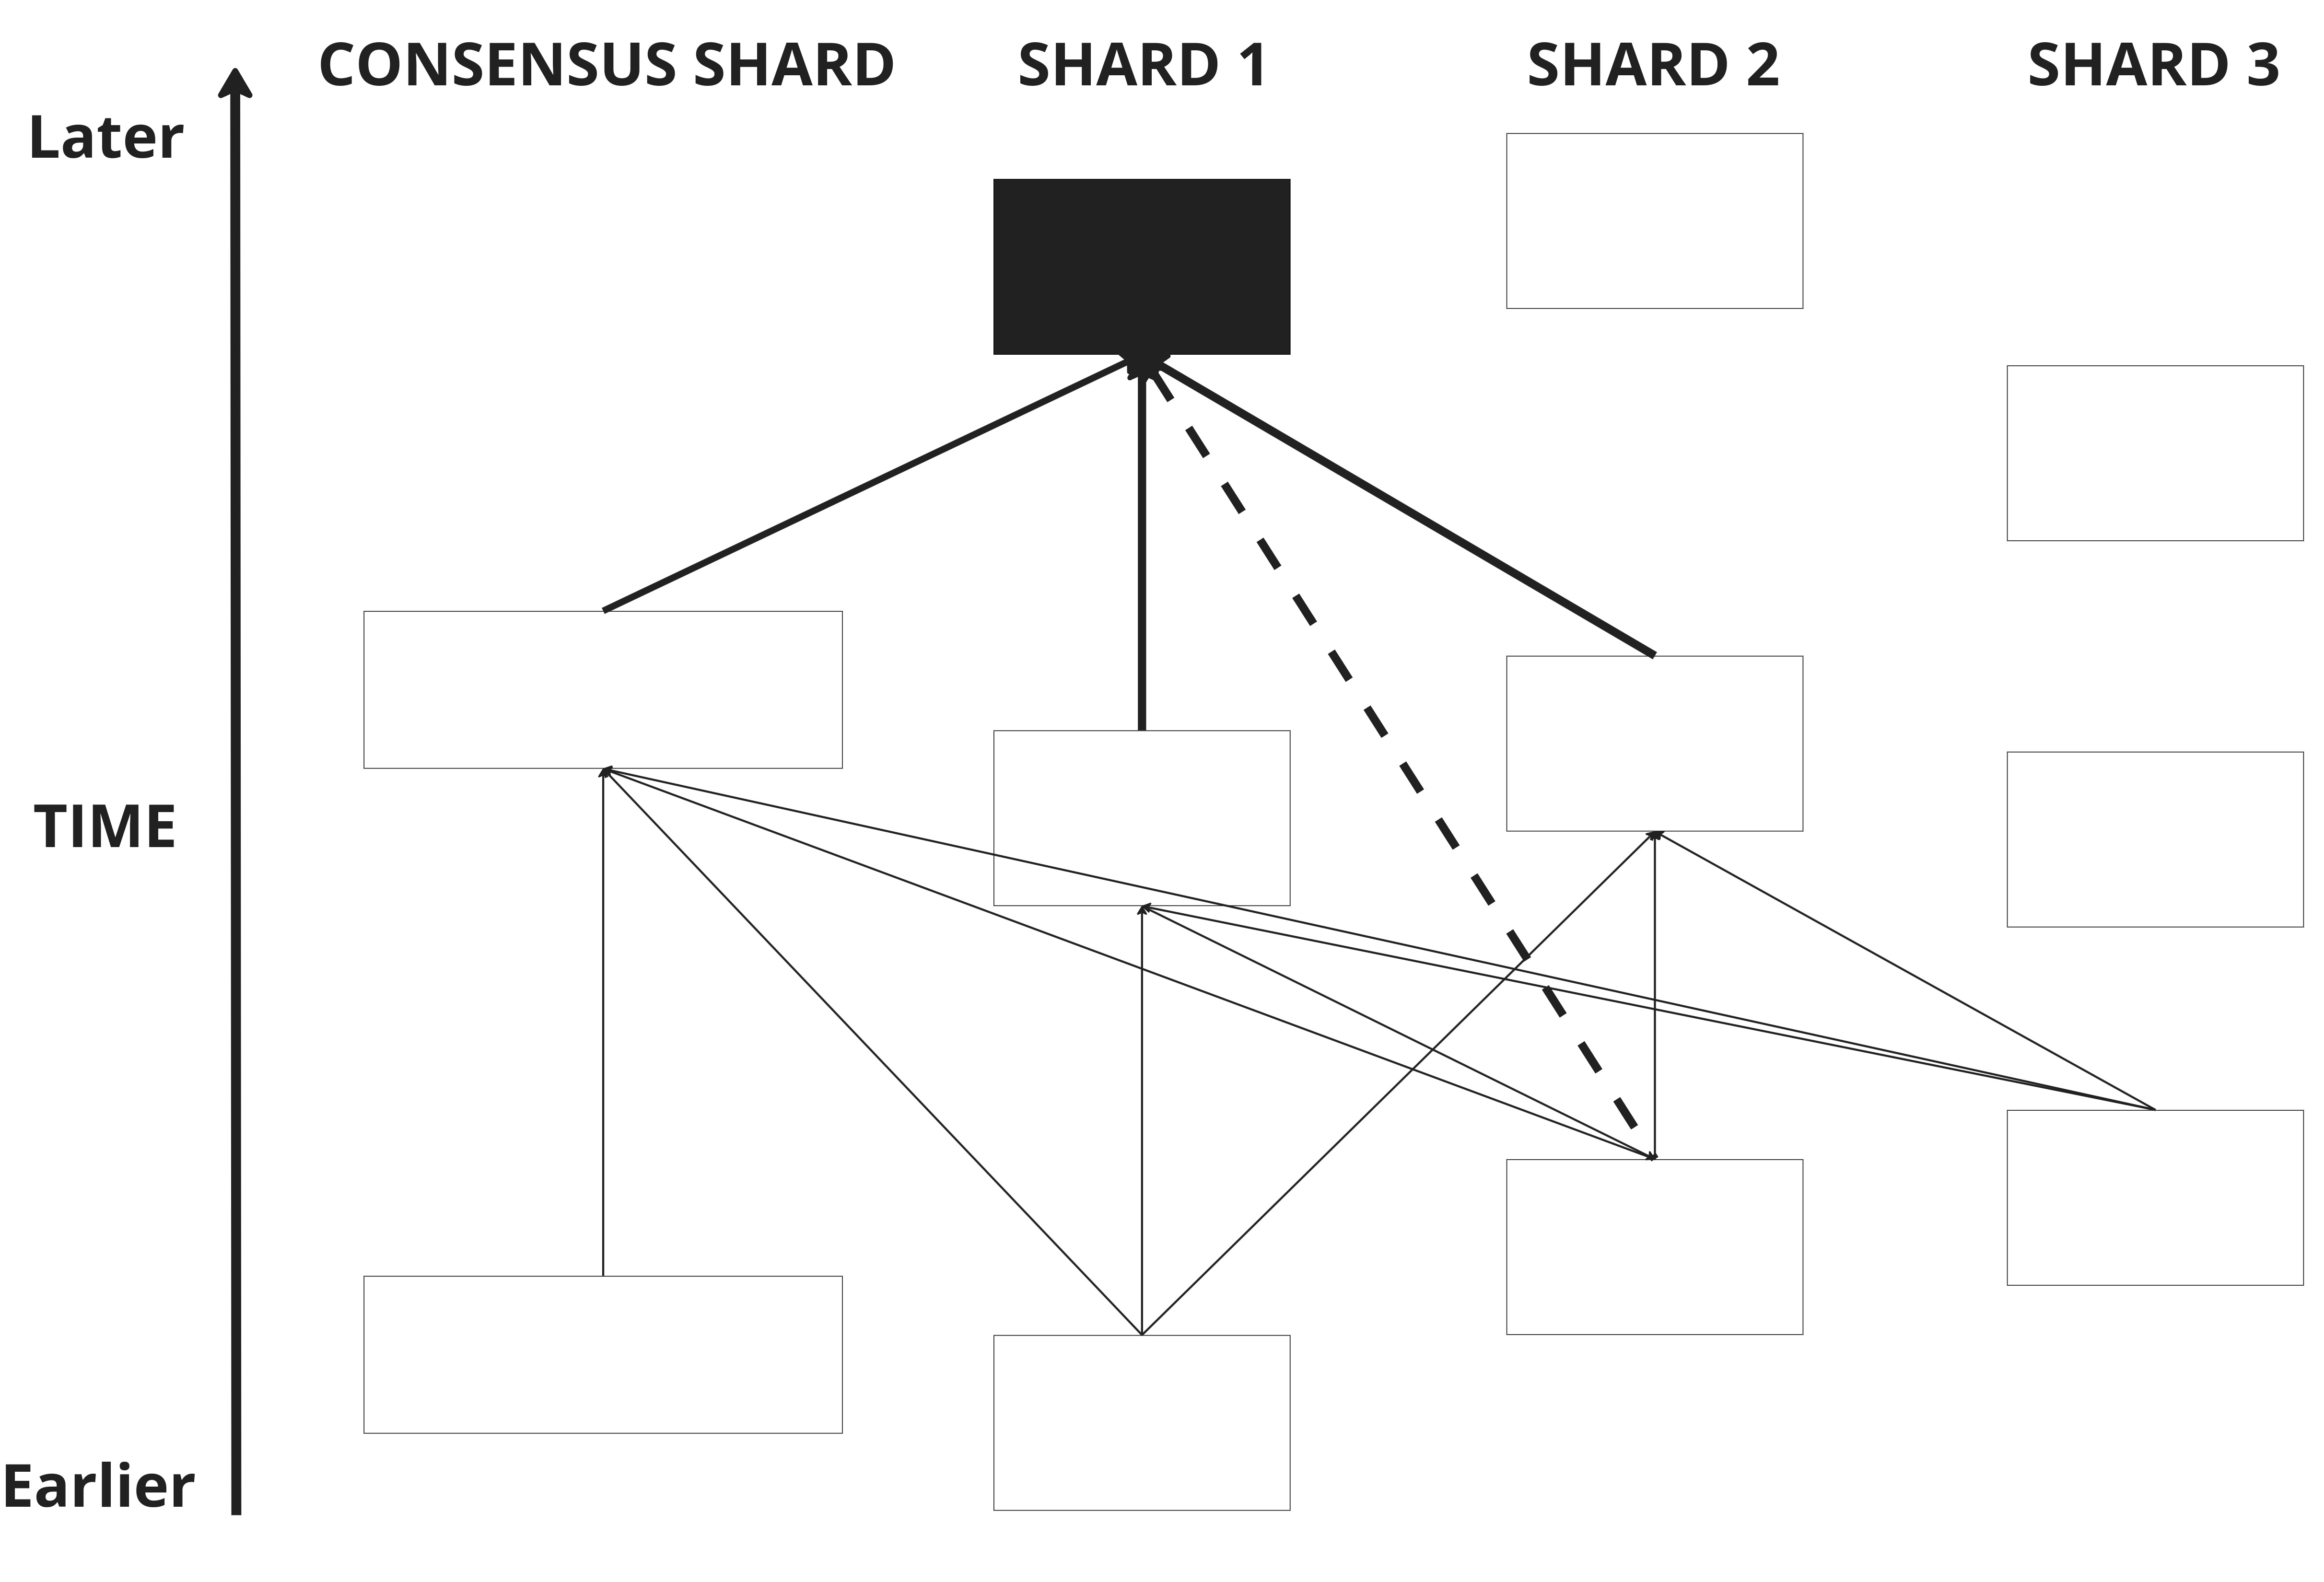
\includegraphics[width=0.5\textwidth]{figures/Subgraph.jpg}
	\caption{ Illustration of a subgraph in the shardDAG. 
		Hashes included in the black block's header are indicated by thick arrows. 
		The dashed arrow is not a valid hash because it is redundant. 
		The black block's entire subgraph is traced by thin arrows.}
	\label{figure:shard-formation}
\end{figure}




\subsubsection{Block Creation}

Validators only propose and sign shard blocks that comply with the shardDAG protocol rules listed below. 
In constructing the shardDAG we refer to a parameter $F$ that controls the branching of the DAG. 
One potential constraint on $F$ is to choose $F$ to be at least the maximum number of malicious shards in the network, limiting the ability of malicious shards to collude with each other and not interact with non-malicious shards. 
However, for performance reasons it may be preferable to use a smaller value of $F$, and potentially vary $F$ amongst the different conditions described below. 
For simplicity, in the descriptions below the single parameter $F$ is retained for all conditions.

\subsubsection{Valid Block Conditions}
For a given shard block $b$ to be valid, it must satisfy all the below conditions:
\begin{itemize}
	\item \textbf{Ordering Condition}: For a shard block $b$ to be valid, $b$'s set of processed CSTs $C$, and processed transactions $T$ must be processed in an order consistent with the order induced by the shardDAG. Specifically, $C$ and $T$ must conform to the following ordering rules. 
	Let $U$ be the set of all (unprocessed) cross-shard transactions in $b$’s subgraph whose destination is $b$'s shard, but which have not been processed in blocks earlier than $b$. 
	Let $V$ be the set of all (unprocessed) cross-shard transactions in $b$’s subgraph whose destination is $b$'s shard, but which have not been processed in $b$ or earlier, i.e. $V=U\setminus C$. 
	The following must be satisfied for $C$ and $T$ to be valid, ordered sets of CSTs and transactions:
	\begin{itemize}
		\item $C$ are the earliest CSTs in $U$. Specifically, for each transaction $c \in C$ there does not exist some other transaction $v \in V$, for which $v$ is ordered earlier than $c$ in the shardDAG.
		\item The ordering of processing of elements of $C$ is consistent with the shardDAG ordering of blocks in which each $c\in C$ was first created.
		\item If a single shard block creates multiple CSTs with shard $b$'s shard as their destination, then the order of their creation is preserved in the order of processing.
		\item $C$ must only contain CSTs that were created within shard blocks in $b$'s subgraph.
		\item $T$ are processed after $C$.
	\end{itemize}
	No rules apply to ordering within sets of transactions and CSTs that are not ordered with respect to each other in the shardDAG, block producers are expected to (but not required to) order based on MEV. 
	
	\item \textbf{Parent Condition}: For a given shard block $b$ with parent shard block $a$ from the same shard, $b$’s subgraph must contain shard blocks created by $>F$ shards that are not present in the subgraph of $a$. 
	Within $b$'s block header, at most one hash to another shard block is allowed per shard, and no hash can fall in the subgraph of another hash (regardless of shard), to eliminate redundant data.
	\item \textbf{Consensus-Parent Condition}: For a given shard block $b$ with parent consensus block $c$, there must not be more than $X$ prior shard blocks from $b$’s shard that also have $c$ as a consensus block parent. 
	$X$ is to be chosen once relative timings of consensus and shard blocks becomes clearer.
\end{itemize}
The purpose of the parent and consensus-parent conditions are to force shards to acknowledge the receipt of shard block headers and outboxes of CSTs.
The purpose of the ordering condition is to force shards to obey a clearly defined order for the processing of transactions and CST that each shard has acknowledged receiving. 
This ordering of transaction and CST processing can be verified and penalties can be applied for breaches of correct ordering.

The following is a central concept in the function of the shardDAG.
When shard $A$ creates a shard block that includes the hash of another shard block $H$, this inclusion acts as an acknowledgement that shard $A$ has received the headers and outboxes of CSTs for $H$ and $H$’s entire subgraph in the shardDAG, up to a limit at which it has been established that this data is no longer required.

An honest validator should not sign a consensus block until it possess the shard block headers and outboxes of CSTs contained within the consensus block.
If a shard block includes a consensus block, or a shard block in its shard block's subgraph, but the creator does not possess the required data, then the shard block risks processing transactions and CSTs in the incorrect order and therefore incurring penalties, and potentially initiating a rollback.


\subsubsection{Shard Block Finalisation Condition}
\label{section:shard-block-finalisation}
The consensus shard incorporates the shardDAG by including sets of shard blocks in each consensus block. 
Let $D$ be the subset of the shardDAG that has been included in consensus blocks. Before a shard block $b\in D$ can be finalised within the consensus chain it must satisfy the following condition
\begin{itemize}
	\item \textbf{Child Condition}: Within $D$, there must be more than $F$ shards that have one or more blocks whose subgraph contains $b$.
\end{itemize}
Note that is not the only condition for a shard block to be finalised, various other conditions must also be met.
The purpose of this child condition is to force shards to distribute their shard block headers and outboxes of CSTs {\it before} they are included in a consensus block, thus constraining the ability of shards to withhold and delay CST processing.



\subsubsection{Local ShardDAG Construction}
Each validator constructs its own local shardDAG as follows
\begin{itemize}
	\item Newly received shard blocks undergo basic validity checks, like checking signatures, checking for more than $F$ shard block hashes etc.
	\item Shard blocks that meet the above basic validity checks are held in a buffer.
	\item Shard blocks are moved from the buffer to the shardDAG 
	\begin{itemize}
		\item When a shard block in a buffer has all of its parents (its shard block hashes) already included in the shardDAG, and 
		\item When the validator has received and verified the shard block's outbox of cross-shard transactions.	
	\end{itemize}
\end{itemize} 
The above ensures that the local shardDAG only includes valid shard blocks and the local shardDAG is not missing any shard blocks such that there are no `holes' in the shardDAG where edges do not have a block on both ends.





\subsection{Global Replication Protocol}
\label{section:global-consensus}

The safety of the system is limited by the safety of the weakest shard committee. 
To address this concern, sharded protocols enhance the sizes of shard committees, 
 thereby achieving acceptable safety guarantees \cite{RapidChain,OmniLedger}.
A similar strategy is employed in zkSharding concept, ensuring that full sharding (encompassing storage, communication, and computation) is not compromised.
That is, within one epoch, validators need to store, process,
 and communicate with only a small part, approximately $\frac{(\log N)^R}{N}$ fraction of the whole system.

As previously stated, the set of shard identifiers \texttt{shardIds} incorporates a metric, 
 the Hamming distance $\texttt{dist}$.
The metric structure of this set is utilized to define a shard's committee: 
 it comprises all validators assigned to the neighborhood of the shard.
$$
\texttt{committee}(\texttt{shardId}) = \bigcup_{
\substack{
\texttt{s} \in \texttt{shardIds}\\
\texttt{dist}(\texttt{s}, \texttt{shardId}) \leq R}}
\texttt{assignment}(\texttt{s}),
$$
Where $R \geq 0$ serves as a protocol parameter that determines the neighborhood's size, 
 the exact value of $R$ is not specified; 
 however, it is selected to ensure the committee size is sufficiently large to afford acceptable safety guarantees.
A standard methodology is employed to estimate the probability of a 1\% attack,
 as detailed in Appendix \ref{appendix:security}.

\begin{remark}
By forming committees in this \emph{local} manner, 
 compatibility between the consensus protocol and the message routing protocol (see Section \ref{section:cross-shard}) is achieved. 
Validators of neighboring shards, tasked with tracking cross-shard messages,
 must retrieve necessary messages from these neighboring shards.
Thus, including them in the consensus committees of neighboring shards addresses the data availability issue.
\end{remark}

The safety analysis, as detailed in \ref{appendix:committee-selection-security}, 
 indicates that the probability of a safety attack is non-negligible if the safety threshold for a shard 
 is set equal to the safety threshold of the entire system.
To address this issue, other widely recognized protocols \cite{OmniLedger,RapidChain} 
 either lower the safety threshold of the entire system or transition to a synchronous network model.
A different solution is proposed here: the adoption of the Multi-Threshold BFT \cite{MultiThresholdBFT} consensus protocol, 
 as described in \ref{section:preliminaries:multi-threshold-bft}, 
 which serves to elevate the safety threshold of the shard. 
The safety threshold, essentially governed by the quorum size, 
 also functions as a safety parameter within the consensus protocol.

Additionally, the zkSharding protocol relies on state transaction proofs (see Section \ref{section:zk}) 
 to enable all validators in the system to verify the state of each shard in a stateless manner. 
However, state transition proofs take time to generate, 
 and standard consensus mechanisms above are used to provide the best security guarantees in the meantime, 
 before the state transition proof is generated.

Therefore, global consensus protocol is a two-level protocol:
\begin{itemize}
    \item \textbf{Local consensus protocol} is a Multi-Threshold BFT consensus protocol, variation of a Sync HotStuf, run by a committee of a shard.
    \item \textbf{Global consensus protocol} is a HotStuff-2 consensus protocol run by the whole validator set.
\end{itemize}

After running the local consensus protocol, each committee leader proposes a block digest along with a quorum certificate to the \mainshard's leader.
The \mainshard's leader collects all block digests and quorum certificates and proposes a block to the \mainshard's committee (whole validator set).
The \mainshard's committee runs a consensus protocol to finalize shards' latest states.

As mentioned, the probability of a safety attack is adjusted by the protocol's safety parameters and is set to be sufficiently low.
However, if the attack still happens, the state of the corrupted accounts is rolled back to the last known good state; for details, see \ref{section:rollbacks}.
Attack detection is facilitated through finalization via state transition proofs, which, once generated, are submitted to the \mainshard.
If the proof is not valid or the \mainshard doesn't receive a state transition proof in a predetermined amount of time (fixed number of successful consensus rounds in the \mainshard),
the committee size of the shard is increased, by increasing the neighborhood size $R$. The consensus protocol is then rerun with the new committee size.


\subsection{Fixing Errors}
\label{section:rollbacks}

The protocol outlines the following stages for state change finalization:
\begin{itemize}
\item Local consensus is achieved.
\item The latest state of the execution shard is provided to the \mainshard.
\item The state transition proof of the execution shard is submitted to the \mainshard.
\item The state transition proof for the zkSharding protocol is submitted to Layer 1.
    Further details on state transition proofs are discussed in Section \ref{section:zk}.
\end{itemize}

Despite the introduction of mechanisms such as 
 the two-level consensus protocol (Section \ref{section:global-consensus}), 
 Multi-Threshold BFT (Section \ref{section:preliminaries:multi-threshold-bft}), 
 and shard committees determined by neighborhood size (Section \ref{section:global-consensus}), 
 there remains a slight chance for malicious nodes to gain control over one of the execution shards.
This can occur before state transition proofs are submitted to the \mainshard, i.e., 
 within minutes of real time. 
To address the potential consequences of such attacks, 
 a rollback mechanism has been integrated into zkSharding.

Rollbacks introduce additional complexity to the protocol and incur a large communication overhead.
However, the expected overhead is negligible due to the low probability of a safety attack.
The protocol follows the following steps before triggering a rollback:

\begin{enumerate}
\item As was mentioned, the shard's state finalization cannot be completed, the corresponding committee size is temporarily increased, and the consensus protocol is rerun on an unsafe state change.
% \todo{Additional slashing conditions should be introduced to discourage stalling proof generation.}
\item If an attack is detected:
\begin{enumerate}
\item Malicious validators who signed an invalid block are slashed.
\item Since the safety of the system is attacked, then the whole validator committee must correct the errors via state rollback.
\end{enumerate}
\end{enumerate}
Regarding the rollback:

\begin{itemize}
\item The most straightforward and robust possibility is to roll back the system to the last known verified state. This solution, however, does not
consider the fact that most of the accounts are not affected by the attack, making redundant the rollback of their states.
\item A more sophisticated approach is to roll back only the affected accounts.
The problem with this approach is that the error propagation speed is higher than the speed of state transition proofs generation,
A big part of the system has to regenerate the latest state transition proofs.
This approach is more complex but suffers from the same problem as the first one.
\end{itemize}

zkSharding uses the first approach with full rollback. 
The details on this will be provided in the future versions of the document.

\subsection{Co-location}
\label{section:colocation}

% \todoisinline{The co-location concept may render fee calculation less understandable for users.}

Cross-shard communication could extend the processing time 
 of applications located on different shards. 
For scenarios demanding the swiftest possible transaction processing (i.e.
increased consistency), the protocol incorporates a \textit{co-location} technique.
\footnote{Obviously, enhancing shard performance leads to improved cross-shard 
performance, but it cannot enable transaction processing within the timings of one replication packet.}

\textit{Co-location} ensures that two accounts $\{a_1, a_2\}$ are consistently 
located within the same shard. 
In other words, $F_S(a_1) = F_S(a_2)$.

The relationship of co-location between addresses $A$ and $B$ 
 is represented as $A \colocate B$. 
The property of transitivity is inherent in the co-location relation, 
 such that if $A \colocate B$ and $B \colocate C$, 
 it logically follows that $A \colocate C$.

\paragraph{Scalability Concerns.} Co-location creates an opportunity for concentrating applications on one shard,
potentially undermining the sharding concept. 
From the perspective of the common good, this approach is counterproductive.
However, for individual actors, co-locating 
applications with those that are most used may seem advantageous. 

To mitigate this, economic limitations on co-location are proposed. 
In essence, an address is permitted to be co-located with at most $N$ other addresses,
 subject to economic constraints that may influence 
 the actual number of feasible co-locations.

 Economic restrictions are applied during the operation of account creation, 
i.e., when a user activates the account with a transaction for the first time.
Typically, this transaction includes funding and initial values.

The details on the restrictions will be provided in the future versions of the document.

% Define the \textit{co-location depth} of an address $A$, 
%  denoted as $|S_A|$, 
% to be the cardinality of the set encompassing all addresses co-located with $A$.
% Formally, $|S_A| = |\bigcup {S \mid S \colocate A}|$.

% Limitations are split into two parts:
% \begin{itemize}
%     \item Economic restrictions. The cost of each co-location depends 
%         on the resulting co-location depth of the address. 
%     \item Ownership or domain restriction. Only addresses controlled 
%         by the same key (potentially a multi-sig key) may be co-located.
% \end{itemize}

% Domain restrictions are introduced to prevent attacks on popular applications
% by malicious users co-locating their addresses with a popular one,
% thereby preventing the addition of new modules by developers. 

% \subsubsection{Economic Restrictions}


% To initialize a previously unmentioned address, 
%  it is necessary to send an initialization transaction to this address,
%  containing initial code, initialization values, and a fee.

% The basic address deployment cost is defined as the sum of 
% the following parameters:
% \begin{itemize}
%     \item Basic transaction fee
%     \item Address activation cost 
%     \item Application bytecode size 
%     \item Constructor call cost
%     \item Reserved data size by the application
%     \item Initial values costs (as part of transaction additional data)
% \end{itemize}

% The co-location's economic restrictions form part of the address creation costs. 
% These costs for address $A$ are defined by the following formula:
% \begin{center}
% \begin{math}
%     \texttt{address\_creation\_fee} = b \cdot k^{|M_A|},
% \end{math}
% \end{center}
% where $b$ represents the basic address creation cost, and $k$ is the co-location multiplier. 
% Both parameters are set in the configuration and can be updated by governance.
% % \footnote{The last defined configuration can be found here: \url{???}.}

% Economic restrictions are applied during the operation of account creation, 
% i.e., when a user activates the account with a transaction for the first time.
% Typically, this transaction includes funding and initial values.

% \subsubsection{Ownership Restrictions}

% The requirement to bind addresses in some manner introduces ownership restrictions.
% These can be implemented in two ways: 
% \begin{itemize}
%     \item Binding solely through an explicit map of co-located addresses. 
%     \item A functional definition of co-located addresses 
%      entails the ability to derive one address from another. 
%      This is possible given that addresses are public keys of some digital signature scheme, 
%      which allows for such derivation.
% \end{itemize}

% In general, it is not feasible to define a "master" key 
% from a derived key. 
% Therefore, an explicit map of bindings must be stored in any case. 
% Furthermore, cryptographic derivation does not add 
% security because forging the map of co-located addresses 
% would require compromising the protocol itself. 
% Thus, the explicit map of the co-located addresses is solely utilized.

% The concept of a \textit{domain} is introduced.
% A domain is a set of co-located addresses defined by the master key.

\paragraph{Binding Map.}

An explicit map can be implemented via an application on top of the 
consensus shard, termed a \textit{co-location manager}. 
Since each validator is required to
 track the consensus shard, 
access to this map is always available. 

% In this scenario, the overall address creation costs become:
%  \begin{center}
%     \begin{math}
%         \texttt{address\_creation\_fee} = b \cdot k^{|M_A|} + e,
%     \end{math}
%     \end{center}
% where $e$ is the execution cost of the co-location manager. 

Co-location manager contains the following operations:
\begin{verbatim}
    class CoLocationManager {
        // Data structure to store co-location domains
        domains: map[address -> array[address]];

        // Function to attempt co-locating two addresses
        co-locate: function(pair<address, address>) -> bool {
            // Checks and updates domains to include the co-location if possible
            // Returns true if co-location is successful, false otherwise
        };

        // Function to release the co-location relationship between two addresses
        release: function(pair<address, address>) -> bool {
            // Updates domains to remove the co-location relationship
            // Returns true if the operation is successful, false otherwise
        };

        // Function to check if two addresses are co-located
        is_co_located: function(pair<address, address>) -> bool {
            // Returns true if the addresses are in the same co-location group, false otherwise
        };

        // Function to calculate the fee for address creation or co-location based on co-location depth
        calculate_fee: function(address) -> number {
            // Calculates and returns the fee based on the co-location depth of the address
        };

        // Function to retrieve the co-location group for a given address
        get_co_location_group: function(address) -> array[address] {
            // Returns the array of addresses that are co-located with the given address
        };
    }
\end{verbatim}

Validators of the shard are tasked with tracking the co-location manager
and processing accounts related to the shard.

Additionally, co-location enables the emulation of a synchronous mode for contract execution.
This means that original Ethereum applications can be redeployed 
 and run on top of \nil without needing to be updated 
 for the asynchronous execution environment of the sharded system.
However, this functionality is a feature of the \nil product 
 and not inherent to the zkSharding architecture,
 so its details are beyond the scope of this document.

% \subsubsection{Merge and Split Operations}

% The split algorithm is determined by the master keys:
% \begin{enumerate}
%     \item Perform the basic split algorithm based on the master keys.
%     \item Define a set of addresses related to the master keys of 
%         each sub-shard. 
% \end{enumerate}

% \subsubsection{Synchronous Execution}
% \todo[inline]{Define if we need it now}
%  \todo[inline]{Could we provide a target for the "local" vs "cross-shard" transactions ratio here? Or may be tell a little bit more about important cases, where colocation is absolutely necessary and be designed for? S.K.}

% Co-location of addresses leads to one more possible UX-related improvement.
% Sharded architecture supposes asynchronous communication between the applications. 
% It influences the development and the resulting bytecode of the contracts. 

% To let seamless migration of the existing applications, we introduce 
%  synchronous execution between the contracts within the same shard. 

% \todo[inline]{Waterfall approach for running transactions within the same shard.}

